% !TEX encoding = UTF-8 Unicode
\subsection{Fase PA: Progettazione Architetturale}
	\textbf{Periodo}: dal \insdate{23}{02}{2015} al \insdate{16}{03}{2015} \\Questa fase comincia con la fine della \insphase{Fase AD} e termina con l'incontro con il proponente per mostrare l'architettura scelta. \\Le attività di questa fase sono:
	\begin{itemize}
		\item \textbf{Norme Di Progetto}: Viene fatto un incremento alle norme per poter stendere il documento \insdoc{Specifica Tecnica v1.0}. Viene successivamente fatta una verifica/validazione per fissare una baseline al documento che diventerà \insfile{Norme Di Progetto v2.0}.
		\item \textbf{Specifica Tecnica}: Questa attività caratterizza la \insphase{Progettazione Architetturale}. Il \insrole{Progettista} stende la \insdoc{Specifica Tecnica} che contiene le scelte progettuali, ad alto livello, che il progetto dovrà avere. Saranno quindi descritti quali design pattern \projectname{} implementerà, l'architettura generale del software, i principali flussi di controllo e il tracciamento dei requisiti.
		\item \textbf{Glossario}: Viene fatto un incremento al Glossario aggiungendo tutti i vocaboli che si ritiene importante siano inclusi. Viene successivamente fatta una verifica/validazione per fissare una baseline al documento che diventerà \insfile{Glossario v3.0}.
		\item \textbf{Piano Di Qualifica}: L'incremento consiste nell'aggiungere al documento \insfile{Piano Di Qualifica v1.0} il dettaglio dell'esito della \insrev{Revisione dei Requisiti} e la parte della pianificazione dei test. Questa attività genererà, dopo una verifica e validazione, il file \insfile{Piano Di Qualifica v2.0}.
		\item \textbf{Piano di Progetto}: l'incremento che sarà fatto al documento \insdoc{Piano Di Progetto} in questa fase consiste nell'apportare correzioni nella divisione delle attività e stillare il consuntivo di questo periodo. Dopo un'accurata verifica che fisserà una nuova baseline e la validazione il documento diventerà \insfile{Piano Di Progetto v2.0}.
	\end{itemize}
	\subsubsection{Diagramma di Gantt delle attività}
	\begin{figure}\centering
		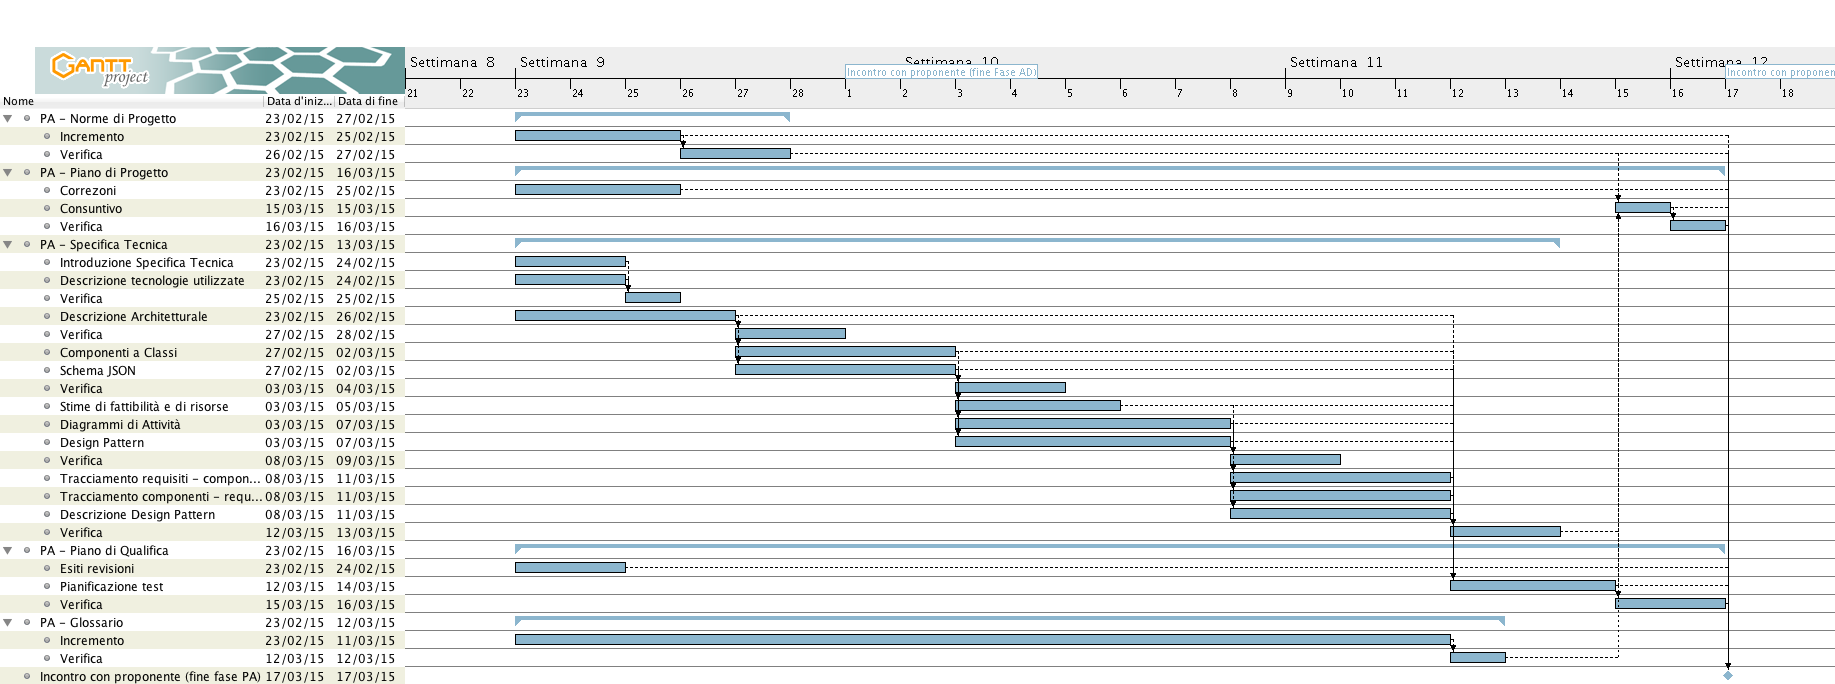
\includegraphics[width=\textwidth]{PianoDiProgetto/Pics/FasePA.png}
	\caption{Gantt Fase PA}
\end{figure}